\chapter{Ultralight Bosons}
\label{chapter:Ultralight Bosons}

\section{Introduction to particle physics}

Particle physics is an area of physics where it's studied the fundamental structure of the universe.  In this work, we are going to use natural units where $c=\hbar=1$, this is to simplify the calculations, and equations, as well use the term Lagrangian instead of Lagrangian density.

\subsection{Symmetries}
Particle physics revolves around the concept of symmetry and symmetry breaking, this concept is also important in mathematics in the area of Group theory.
Symmetry is a property of an object, that under a certain operation the object remains the same. We define those operations as a group.

\subsubsection{Continuous symmetries}
Certain symmetries are composed of continuous operations, for example, rotating a circle by an angle, it doesn't matter which angle we choose, the object suffers no change.

Noether's theorem says that \cite{Noether1918},
\textit{The invariance of the Lagrangian $\mathcal{L}$ under a continuous symmetry implies the existence of a conserved quantity.}

Taking into account the Noether's theorem, it's possible to verify:
\begin{itemize}
	\item Space-time symmetry:
	They result in energy-momentum conservation and are characterized by the Poincaré group. Inferred from this law as conserved quantities or charges are energy, linear momentum, and total angular momentum. 
	\item Internal symmetry:
	Is a symmetry acting on fields, these can be global, independent of the space-time point, and local, dependant on the space-time point, the latter  are known as gauge symmetries. Where the internal particle charges emerge, electric charge, hypercharge, weak spin or colour charge.
	The quantity usually conserved is current-density
\end{itemize}


\subsection{U(1) symmetry}

In this section, we are going to use the Klein-Gordon equation to prove the gauge symmetry, note that we can use the Dirac equation
\begin{equation}
	\label{KG}
	(\Box + m^2)\phi = 0\,,
\end{equation}
where $\phi$ is a scalar field \cite{grif} and $\Box=\left(\frac{\partial^2}{\partial t^2}-\nabla^2\right)$.

Let us consider the Klein-Gordon Lagrangian for a free complex scalar
\begin{equation}
	\label{lKG}
	\mathcal{L}_{KG}(\phi,\partial_\mu\phi)=K-V=g^{\mu\nu}\partial_\mu\phi^*\partial_\nu \phi - m^2 \phi^*\phi\,,
\end{equation}
where $K$ and $V$ are the kinetic and potential term, respectively, $\partial_\mu=\frac{\partial}{\partial x_\mu}=(\frac{\partial}{\partial t},-\vec{\nabla})$, and $g^{\mu\nu}=diag(+,-,-,-)$ is the Minkowski metric.
\subsubsection{Global symmetry}
Let's introduce the following global phase transformation
\begin{equation}
	\label{GPT}
	\phi\rightarrow \phi'=e^{-iq\alpha}\phi\,,
\end{equation}
where $\alpha$ is a global parameter, global as in it's equal at every space-time point, and $q$ 
represents the charge of the scalar field.

The Lagrangian in \autoref{lKG} gets transformed to
\begin{align}
	\label{tlKG}
	\begin{array}{lll}
			\mathcal{L}_{KG}(\phi',\partial_\mu\phi')&=g^{\mu\nu}\partial_\mu(e^{iq\alpha}\phi^*)\partial_\nu(e^{-iq\alpha}\phi) - m^2 (e^{iq\alpha}\phi^*)(e^{-iq\alpha}\phi) \\
			&=g^{\mu\nu}\partial_\mu\phi^*\partial^\nu \phi - m^2 \phi^*\phi \\
			&=\mathcal{L}_{KG}(\phi,\partial_\mu\phi)\,,
	\end{array}
\end{align}
and so we conclude that the Klein-Gordon Lagrangian remains invariant under a global phase transformation.
So we see that \autoref{GPT} is actually a unitary transformation of one dimension, and this class of groups are denoted as $U\textrm{(1)}$ symmetries. 

\subsubsection{Local symmetry}

Let us consider the same Lagrangian as in \autoref{lKG}, but now we replace the global parameter, with a local one, $\alpha(x^\mu)$, which depends on the space-time point defined by
\begin{equation}
	\phi \rightarrow \phi'=e^{-iq\alpha(x^\mu)}\phi\,
\end{equation}
we get
\begin{align}
	\begin{array}{lllll}
		\mathcal{L}_{KG}(\phi',\partial_\mu\phi')&=g^{\mu\nu}\partial_\mu(e^{iq\alpha(x^\mu)}\phi^*)\partial_\nu(e^{-iq\alpha(x^\mu)}\phi) - m^2 (e^{iq\alpha(x^\mu)}\phi^*)(e^{-iq\alpha(x^\mu)}\phi) \\
		&=g^{\mu\nu}(iq\partial_\mu\alpha(x^\mu)e^{iq\alpha(x^\mu)}\phi^*+e^{iq\alpha(x^\mu)}\partial_\mu\phi^*)\times \\ 
		&(-iq\partial_\nu\alpha(x^\mu)e^{-iq\alpha(x^\mu)}\phi+e^{-iq\alpha(x^\mu)}\partial_\nu\phi) - m^2\phi^*\phi \\
		&=\mathcal{L}_{KG}(\phi,\partial_\mu\phi)+q^2g^{\mu\nu}\partial_\nu\alpha(x^\mu)\partial_\nu\alpha(x^\mu)\phi^*\phi \\
		&-iqg^{\mu\nu}e^{iq\alpha(x^\mu)}\partial_\mu\phi^*\partial_\nu\alpha(x^\mu)\phi+iqg^{\mu\nu}e^{-iq\alpha(x^\mu)}\partial_\nu\phi\partial_\mu\alpha(x^\mu)\phi^*\,,
	\end{array}
\end{align}
therefore we see that the free Klein-Gordon theory is by no means $U\textrm{(1)}$ invariant.

Let's assume that gauge invariance is a fundamental law of the universe, the way we make our theory invariant is by redefining our partial derivative.
A gauge transformation is not expected to modify any observable values, observable quantities should not be directly dependent on the field's derivative.
Instead, we propose replacing the partial derivatives with the gauge covariant derivative 
\begin{equation}
	\label{pd1}
	\partial_\mu\rightarrow\mathcal{D}_\mu =\partial_\mu+V_\mu\,.
\end{equation}

The condition that guarantees the theory to be invariant is given by
\begin{equation}
	\label{invariancecondition}
	(\mathcal{D}_\mu \phi)'=e^{-iq\alpha(x)}\mathcal{D}_\mu \phi\,,
\end{equation}
using the \autoref{pd1} and \autoref{invariancecondition} we get
\begin{align}
	\begin{array}{ll}
		(\mathcal{D}_\mu \phi)'=(\partial_\mu+V_\mu')\phi'&=e^{-iq\alpha(x^\mu)}\left[\partial_\mu+V_\mu'-iq\partial_\mu\alpha(x^\mu)\right]\phi =e^{-iq\alpha(x^\mu)}\mathcal{D}_\mu \phi \\
		& \Leftrightarrow \mathcal{D}_\mu=\partial_\mu+V_\mu'-iq\partial_\mu\alpha(x^\mu)\,,
	\end{array}
\end{align}
and making $V_\mu=iqA_\mu$, where $A_\mu$ is a gauge field and using \autoref{pd1}, we can see that
\begin{equation}
	\label{gaugefieldchange}
	A_\mu'=A_\mu+\partial_\mu\alpha(x^\mu)\,,
\end{equation}
and so we can now define the covariant derivative, as
\begin{equation}
	\label{covdev}
	\mathcal{D}_\mu = \partial_\mu + iqA_\mu\,.
\end{equation}

Note that this gauge covariant derivative will remain unchanged whenever we apply a gauge transformation since the change in the partial derivative will now be balanced out by the change in the gauge field. The gauge covariant derivative can be explained intuitively as a means to alter the derivative operator so that the outcome is unaffected by a gauge transformation.
This is crucial since a gauge transformation is meant to restore the system to its initial condition while merely changing the arrangement of unobservable degrees of freedom.

Another approach is using the "kinetic"\ term in \autoref{lKG}, it relates to the field propagator and it defines how the particle moves in empty space.
The translation is generated by the derivative, and a finite translation is constructed by repeatedly applying infinitesimal translations.
The consequence is to create an infinitesimal phase change that goes along with each infinitesimal translation when the partial derivative is replaced by the gauge covariant derivative.
As a result, a phase shift is present along with a finite translation. 

\subsubsection{Spontaneous symmetry breaking}
The mechanism of SSB is one of the most potent concepts in current theoretical physics.
It serves as the foundation for the majority of recent advances in the statistical mechanics description of phase transitions as well as the description of collective events in solid state physics.
Additionally, it has made it possible to combine electromagnetic, weak, and strong interactions in elementary particle physics.
Philosophically, the concept is exceedingly complex and nuanced (which is partly why its successful application is a relatively recent accomplishment), and popular explanations of it fall short of doing it credit. 

The usual, cheap explanation for this phenomenon is that it results from the presence of an asymmetrical absolute minimum, or "ground state", which is shown in the \autoref{fig:SSB}, for the potential, $V(\phi)=\alpha |\phi|^2+\beta|\phi|^4$

\begin{figure}[H]
    \centering
	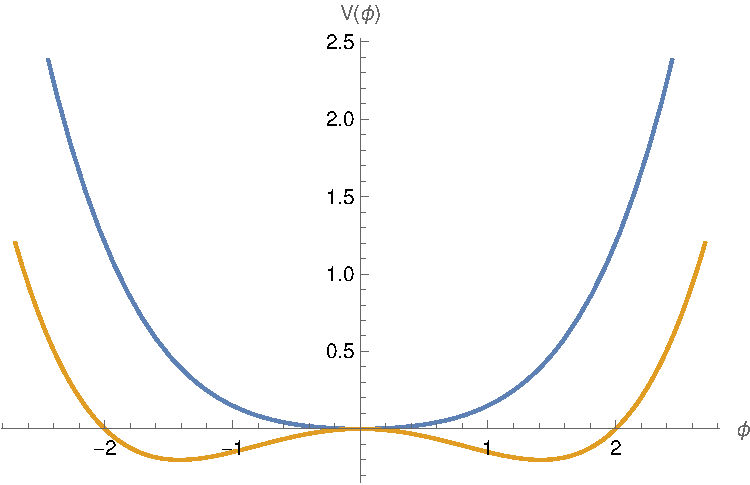
\includegraphics[width=0.7\linewidth]{graphs/SSB.pdf}
	\caption{Example of a Spontaneous symmetry breaking, with the blue line representing the symmetrial ground state ($\alpha>0$,$\beta>0$), and the orange line representing the asymmetrical ground state ($\alpha<0$,$\beta>0$).}
	\label{fig:SSB}
\end{figure}
\noindent This symmetry breaking occurs when we change the sign of the coupling terms of the interactions.

The main advantage of this symmetry breaking is due to the Goldstone theorem \cite{grif}, which says
\label{goldstone}

\textit{spontaneous breaking of a continuous
global symmetry is always accompanied by the appearance of one or more massless scalar
(spin-0) particles}.

\section{Bosonic sector}

In this section, we are going to take a quick look at the theory invariant under the symmetry $\textrm{SU}(2)_W \times  \textrm{U}(1)_Y$, denoted as ElectroWeak symmetry (EW) \cite{grif} \cite{Freitas_2021}.
Let the Higgs potential scalar be given by,
\begin{equation}
	V_0(H)=\mu_{H}^{2}H^{\dag}H+\frac{1}{2}\lambda_H(H^{\dag}H)^2\,,
\end{equation}
where $H$ is the Higgs field, a SU$(2)_W$ complex scalar doublet, and is written as
\begin{equation}
	H=\frac{1}{\sqrt{2}}
	\left(\begin{array}{c} w_1+iw_2 \\ v_h+h+iz \end{array} \right)\,,
\end{equation}
where $v_h$ is the vacuum expectation value VEV which describes the classical ground state of the theory, $v_h\simeq$ \SI{246}{G\eV}, $h$ represents the radial fluctuations. When a SSB occurs, due to the Higgs doublet 
\begin{equation}
	\langle H \rangle = \frac{1}{\sqrt{2}}\left(
	\begin{array}{c}
	0 \\
	v_h
	\end{array}\right)\,
\end{equation}
the goldstone modes $w_{1,2}$, that appear due to the Goldstone Theorem \ref{goldstone}, and z are absorved by the longitudinal degrees of freedom of the $W^{\pm}$ and $Z$ gauge bosons.

The kinetic term of the Lagrangian, between the coupling of EW vector bosons with the Higgs doublet, is
\begin{equation}
	\mathcal{L}_{kin}\supset(\mathcal{D}_\mu H^\dag) (\mathcal{D}^\mu H)\,,
\end{equation}
where $D_\mu$ is the covariant derivative, which is defined by
$\mathcal{D}_\mu=\partial_\mu+ig_1\frac{\sigma_a}{2}A_\mu^a+ig_2YB_\mu 
$, $g_{1,2}$ are the U$(1)_Y$ and SU$(2)_W$ gauge couplings, $Y$ is the hypercharge, $\sigma_a$ ($a$ = x,y,z) are the Pauli matrices, and the $B_\mu$, $A_\mu^a$ the massless EW gauge bosons.

\section{Ultralight complex scalar}
This section serves as a simple example of how we can obtain an ultralight particle.
The model in question will contain an additional complex singlet $\phi$ charged under a global U$(1)_G$ symmetry, such that it is invariant under the global phase transformation, $\alpha$, \cite{Freitas_2021}
\begin{equation}
	\phi \rightarrow e^{i\alpha}\phi\,.
\end{equation}

The potential under this new complex singlet, before the electroweak symmetry breaking (EWSB), is defined as
\begin{equation}
	\label{potential}
	V(H,\phi)=V_0(H)+ \mu_\phi^2\phi^*\phi+\frac{1}{2}\lambda_\phi|\phi^*\phi|^2+\lambda_{H\phi}H^{\dag}H\phi^*\phi\,,
\end{equation}
where $\lambda_{H\phi}$, is commonly known as the Higgs portal coupling, the coupling term between the boson scalar and the Higgs doublet.

The conditions which allow us to have a SSB are
\begin{equation}
	\label{couplingtermconditions}
	\lambda_H,\lambda_\phi>0 \quad \textrm{and} \quad \lambda_H\lambda_\phi-\lambda_{H\phi}^2>0\,,    
\end{equation}
they allow us to write $\mu_H^2=-\lambda_Hv_h^2$, this $\mu_H^2$ appears as a consequence of the minimum of the potential, and the Hessian matrix of \autoref{potential} and replacing $\mu_H^2$, this matrix contains the mass terms and reads as \cite{Freitas_2021}
\begin{equation}
	M^2=\left( \begin{array}{cccc} 
		0_{3\times3} & 0_{3\times1} & 0_{3\times1} & 0_{3\times1} \\
		0_{1\times3} & 2\lambda_Hv_h^2 & 0 & 0 \\
		0_{1\times3} & 0 & \mu_\phi^2+\frac{1}{2}\lambda_{H\phi}v_h^2 & 0 \\
		0_{1\times3} & 0 & 0 & \mu_\phi^2+\frac{1}{2}\lambda_{H\phi}v_h^2
	\end{array}\right)\,.
\end{equation} 

This matrix is already in the diagonal form so it's not needed to be diagonalized and so we can see that there is a Goldstone boson, the masses of the SM-Higgs boson and 2 new complex scalar particles are given by
\begin{equation}
	m_h^2=2\lambda_Hv_h^2 \quad \quad \quad m_\phi^2=\mu_\phi^2+\frac{1}{2}\lambda_{H\phi}v_h^2\,.
\end{equation}
The relevant interactions with the singlet $\phi$ are given by
\begin{equation}
	\lambda_{h\phi\phi}=v_h\lambda_{H\phi}\,, \quad \quad
	\lambda_{hh\phi\phi}=\lambda_{H\phi}\,, \quad \quad
	\lambda_{\phi\phi\phi\phi}=\lambda_\phi\,.
\end{equation}

This model can allow an ultralight complex scalar, it can be obtain via a feebly interacting scenario, which consists of making the portal coupling very small, $10^{-42}\gtrsim \lambda_{H\phi} \gtrsim 10^{-62}$, and so the mass of our complex scalar $\phi$ gets around, $10^{-10}\gtrsim m_{\phi} \gtrsim 10^{-20}$ \si{\eV} \cite{Freitas_2021}.

\section{Real pseudo-Goldstone Boson}

In the previous section, we took a look at complex scalars (and their advantages). However real scalars also have quite a bunch of interesting advantages. 
Let's begin by considering the same potential as in \autoref{potential}, and that not only the Higgs doublet develops a VEV but also the $\phi$ scalar, $v_\sigma$. But now that we break the U$(1)_G$ symmetry, due to Goldstone's theorem, a new massless real scalar emerges in the physical particle spectrum.
However evidence shows that this isn't enough to get anywhere, so let us take a look at the introduction of a small soft symmetry breaking such that \cite{Freitas_2021}
\begin{equation}
	\label{vsoft}
	V(H,\phi)\rightarrow V(H,\phi)+V_{soft}\,, \quad \quad \textrm{where} \quad \quad V_{soft}=\frac{\mu_s^2}{2}(\phi^2+\phi^{*2})\,,
\end{equation}    
the $V_{\textrm{soft}}$ scalar potential is used as an explicit symmetry breaking, and it occurs when we introduce an external term in our theory which will turn our theory invariant, this will helps us to give mass to our Goldstone boson, from the SSB, and we call this new Golstone Boson, pNGB.

The Goldstone mode can be described as a phase, $\theta$, and so the $\phi$ scalar can be expressed as
\begin{equation}
	\phi=\frac{1}{\sqrt{2}}(\sigma+v_\sigma)e^{i\theta/v_\sigma}\,,
\end{equation}
with $\sigma$ denoting quantum fluctuations in the radial directions around the classical field, $v_\sigma$. And so our $V_\textrm{soft}$ scalar potential in \autoref{vsoft} can be written as 
\begin{equation}
	\label{newvsoft}
	V_\textrm{soft}=\dfrac{\mu_s^2}{2}(\sigma+v_\sigma)^2\cos\left(\dfrac{2\theta}{v_\sigma}\right)\,.
\end{equation}


Thus our degrees of freedom are $\sigma$, $h$, and $\theta$, and so let's determine the minimization conditions taking
\begin{equation}
	\frac{\partial V}{\partial \sigma}=\frac{\partial V}{\partial h}=\frac{\partial V}{\partial \theta}=0 \Leftrightarrow \left\{\begin{array}{c}
		\mu_H^2=-\frac{1}{2}(v_h^2\lambda_H+v_\sigma^2\lambda_{H\phi}) \\
		\mu_\phi^2=-\frac{1}{2}(v_\sigma^2\lambda_\phi+v_h^2\lambda_{H\phi}+2\mu_s^2)
	\end{array} \right. \,,
\end{equation}
where $\theta=n\pi v_\sigma \textrm{ and } h=\sigma=0$.

The corresponding Hessian matrix is defined by
\begin{equation}
	M^2=\left(\begin{array}{ccc}
		\dfrac{\partial^2V}{\partial h^2} & \dfrac{\partial^2V}{\partial h \partial\sigma} & \dfrac{\partial^2V}{\partial h \partial\theta} \\ [8pt]
		\dfrac{\partial^2V}{\partial \sigma \partial h} & \dfrac{\partial^2V}{\partial \sigma^2} & \dfrac{\partial^2V}{\partial \sigma \partial\theta} \\ [8pt]
		\dfrac{\partial^2V}{\partial \theta \partial h} & \dfrac{\partial^2V}{\partial \theta \partial\sigma} & \dfrac{\partial^2V}{\partial\theta^2}
	\end{array}\right)=\left(\begin{array}{ccc}
		v_h^2\lambda_H & v_hv_\sigma\lambda_{H\phi} & 0 \\
		v_hv_\sigma\lambda_{H\phi} & v_\sigma^2\lambda_\phi & 0 \\
		0 & 0 & -2\mu_s^2\,,
	\end{array}\right)
\end{equation}
notice that the matrix isn't diagonalized, so let's rotate the matrix to the physical basis, where we can more easily see the physical particle spectrum, we obtain
\begin{equation}
	m^2=U^\dag M^2 U = \left(\begin{array}{ccc}
		m^2_{h_1} & 0 & 0 \\
		0 & m^2_{h_2} & 0 \\
		0 & 0 & m^2_{\theta}
	\end{array}\right)\,,
\end{equation}
where the eigenvalues are
\begin{equation}
\label{masses}
	\begin{array}{c}
		m^2_{h_{1,2}}=\frac{1}{2}\left[v_h^2\lambda_H+v_\sigma^2\lambda_\phi\mp\sqrt{v_h^4\lambda_H^2+v_\sigma^4\lambda_\phi^2+2v_h^2v_\sigma^2(2\lambda_{H\phi}^2-\lambda_H\lambda_\phi)}\right] \\ 
		m^2_\theta=-2\mu_s^2\,,
	\end{array}
\end{equation}
where $U$ is the matrix containing the eigenvectors, which can be expressed as a matrix rotation and reads as
\begin{equation}
	U=\left(\begin{array}{lll}
		\cos(\alpha) & \sin(\alpha) & 0 \\
		-\sin(\alpha) & \cos(\alpha) & 0 \\
		0 & 0 & 1
	\end{array}\right)\,,
\end{equation}
where $\alpha$, is the mixing angle.
The physical basis vectors $h_1$ and $h_2$ can be represented in terms of the gauge eigenbasis ones $h$ and $\sigma$, as follows
\begin{equation}
\label{mixing}
	\left(\begin{array}{l}
		h_1 \\
		h_2 \\
		\theta 
	\end{array}\right)=U\left(\begin{array}{l}
	h \\
	\sigma \\
	\theta 
\end{array}\right)\Leftrightarrow \left\{\begin{array}{cc}
     h=\cos(\alpha)h_1-\sin(\alpha)h_2 \\
     \sigma=\sin(\alpha)h_1+\cos(\alpha)h_2 
\end{array}\right.\,,
\end{equation}

When expanding the "kinetic"\ term of the scalar field, we get
\begin{equation}
    \partial_\mu\phi^*\partial^\mu\phi=\dfrac{1}{2}\left[(\partial\sigma)^2+(\partial\theta)^2\dfrac{(\sigma+v_\sigma)^2}{v_\sigma^2}\right]\,,
\end{equation}
we are able to notice that there is the appearing of cubic interacting between $\sigma\theta\theta$ from $(\partial\theta)^2\sigma$, using $\autoref{mixing}$, it reads as
\begin{equation}
\label{sigmathetatheta}
    (\partial\theta)^2\sigma=-\dfrac{1}{2}\left[\sin(\alpha)m_{h_1}^2h_1+\cos(\alpha)m_{h_2}^2h_2\right]\theta^2+\sigma m_\theta^2\theta^2\,.
\end{equation}

Notice that in \autoref{newvsoft} expanding the cosine with a Taylor series, $\cos(x)\simeq 1-\dfrac{x^2}{2}$, will get us
\begin{equation}
\label{taylorcosine}
	\cos\left(\dfrac{2\theta}{v_\sigma}\right)\simeq 1 - \dfrac{2\theta^2}{v_\sigma}\,,
\end{equation}
this also means that the theory is invariant under a $Z_2 \in U\textrm{(1)}_G$ symmetry where the pNGB transforms as $\theta \rightarrow -\theta$.
With this new expansion we can see that the soft breaking potential, in \autoref{newvsoft}, forms a cubic coupling term $\dfrac{m_\theta^2}{v_\sigma^2}\sigma\theta^2$, which will cancel out with the last term from \autoref{sigmathetatheta}.

Note that the mixture of $h$ and $\sigma$, allows for the appearance of a partial width decay of the Higgs like particles, $h_1$ or $h_2$, into $\theta\theta$, in \autoref{sigmathetatheta}, being $\Gamma(h_i\rightarrow\theta\theta)\propto U_{1i}^2/v_\sigma^2$, the initial constraint for the mixing angle, backed up by experiments, is $|\sin(\alpha)| < 0.3$ \cite{robens2021extended}, and as the value of $|\sin(\alpha)|$ decreases, the probability of $h_1$ decaying into $\theta\theta$ decreases as well, but the probability of $h_2$ decaying into $\theta\theta$ increases. Later in this work this will become relevant.

This approach provides three real scalars.
First, one of the Higgs bosons, either $h_1$ or $h_2$, must be the SM-like Higgs, whereas the other can be heavier or lighter than \SI{125}{G\eV}.
Second, the pNGB $\theta$ derives its mass from a soft-breaking parameter and is a candidate for a real scalar with an ultralight mass. Its mass comes from a minor violation of the global $U\textrm{(1)}_G$ symmetry\cite{Freitas_2021}. 

The expansion in \autoref{taylorcosine} allows us to see the appearance of interactions with $\theta$, and the cubic and quartic coupling terms of these interactions are \cite{Freitas_2021}
\begin{align}
	\label{couplingterms}
	\begin{array}{lll}
	&\lambda_{\theta\theta h_i}=\dfrac{m_{h_1}^2}{v_\sigma}U_{2i}\,,\\	[8pt]
	&\lambda_{\theta\theta h_i h_j}=\dfrac{1}{4}\left[\lambda_\phi U_{2i}U_{2j}+(-1)^{i+j}\lambda_{H\phi}U_{1i}U_{1j}\right]\,,\\ [8pt]
	&\lambda_{h_i SM SM}=U_{1i}g_{SM}\,.
	\end{array}
\end{align}

In terms of these parameters, the quartic terms can be stated as follows
\begin{align}
 \label{couplingtermsfrominteraction}
 \begin{array}{lll}
 	&\lambda_{H\phi}=\dfrac{\sin(2\alpha)(m_{h_1}^2-m_{h_2}^2)}{2v_\sigma v_h}\,, \\[8pt]	
 	&\lambda_{\phi}=\dfrac{\cos^2(\alpha)m_ {h_2}^2+\sin^2(\alpha)m_{h_1}^2}{v_\sigma^2}\,, \\[8pt]
 	&\lambda_{H}=\dfrac{\cos^2(\alpha)m_ {h_1}^2+\sin^2(\alpha)m_{h_2}^2}{v_h^2}\,.
 \end{array}
\end{align}
And the quartic self-interaction of the pNGB is
\begin{equation}
	\lambda_{\theta\theta\theta\theta}=-\dfrac{m_\theta^2}{6v_\sigma^2}\,.
\end{equation}

Note that $\lambda_{H\phi}$ has to be small due to the radiative corrections, this is not the main topic of this work, for more information on the subject check \cite{Freitas_2021}.